\documentclass[a4paper,11pt]{report}
 
% Import des extensions
\usepackage[T1]{fontenc}
\usepackage[utf8]{inputenc}
\usepackage[francais]{babel}
\usepackage{graphicx}
\usepackage{color}
\usepackage[table]{xcolor}
\usepackage{colortbl}
\usepackage{geometry}
\usepackage{hyperref}
\usepackage{fullpage}
\usepackage{listings}
\usepackage{eso-pic}
\usepackage[nottoc]{tocbibind}
\geometry{hmargin=2.5cm,vmargin=3.5cm}

%\lstset{numbers=left, stepnumber =1, firstnumber =1, numberfirstline=true, frame=lines}

\definecolor{darkWhite}{rgb}{0.94,0.94,0.94}

\lstset{
  aboveskip=3mm,
  belowskip=-2mm,
  backgroundcolor=\color{darkWhite},
  basicstyle=\footnotesize,
  breakatwhitespace=false,
  breaklines=true,
  captionpos=b,
  commentstyle=\color{red},
  deletekeywords={...},
  escapeinside={\%*}{*)},
  extendedchars=true,
  framexleftmargin=16pt,
  framextopmargin=3pt,
  framexbottommargin=6pt,
  frame=tb,
  keepspaces=true,
  keywordstyle=\color{purple},
  literate=
  {²}{{\textsuperscript{2}}}1
  {⁴}{{\textsuperscript{4}}}1
  {⁶}{{\textsuperscript{6}}}1
  {⁸}{{\textsuperscript{8}}}1
  {€}{{\euro{}}}1
  {é}{{\'e}}1
  {è}{{\`{e}}}1
  {ê}{{\^{e}}}1
  {ë}{{\¨{e}}}1
  {É}{{\'{E}}}1
  {Ê}{{\^{E}}}1
  {û}{{\^{u}}}1
  {ù}{{\`{u}}}1
  {â}{{\^{a}}}1
  {à}{{\`{a}}}1
  {á}{{\'{a}}}1
  {ã}{{\~{a}}}1
  {Á}{{\'{A}}}1
  {Â}{{\^{A}}}1
  {Ã}{{\~{A}}}1
  {ç}{{\c{c}}}1
  {Ç}{{\c{C}}}1
  {õ}{{\~{o}}}1
  {ó}{{\'{o}}}1
  {ô}{{\^{o}}}1
  {Õ}{{\~{O}}}1
  {Ó}{{\'{O}}}1
  {Ô}{{\^{O}}}1
  {î}{{\^{i}}}1
  {Î}{{\^{I}}}1
  {í}{{\'{i}}}1
  {Í}{{\~{Í}}}1,
  morekeywords={*,...},
  numbers=left,
  numbersep=10pt,
  numberstyle=\tiny\color{black},
  rulecolor=\color{black},
  showspaces=false,
  showstringspaces=false,
  showtabs=false,
  stepnumber=1,
  stringstyle=\color{gray},
  tabsize=4,
  title=\lstname,
}

\newcommand{\blap}[1]{\vbox to 0pt{#1\vss}}
\newcommand\AtUpperLeftCorner[3]{%
\put(\LenToUnit{#1},\LenToUnit{\dimexpr\paperheight-#2}){\blap{#3}}%
}
\newcommand\AtTopCenterPage[2]{%
\put(\LenToUnit{.5\paperwidth},\LenToUnit{\dimexpr\paperheight-#1}){\blap{\hbox to 0pt{\hss#2\hss}}}%
}
\newcommand\AtUpperRightCorner[3]{%
\put(\LenToUnit{\dimexpr\paperwidth-#1},\LenToUnit{\dimexpr\paperheight-#2}){\blap{\llap{#3}}}%
}


\author{Dylan Bideau, Julien Turpin, Pierre Bogrand, Guillaume Vincenti}
\title{\huge{Nautilus - Rapport}}
\date{10 Avril 2018}

\begin{document}
\makeatletter
\begin{titlepage}

	\AddToShipoutPicture{
		\AtUpperLeftCorner{1.5cm}{1cm}{
\includegraphics[width=4cm]{Photos/ensea.png}}
	}
	\begin{center}
		\vspace*{10cm}
		\textsc{\@title}
		\vspace*{0.5cm}
		\hrule
		\vspace*{0.5cm}
		\large{\@author}
	\end{center}
	\vspace*{9.2cm}
	\begin{center}
		\large{\@date}
	\end{center}
\end{titlepage}
\ClearShipoutPicture

\renewcommand{\contentsname}{Sommaire}
\tableofcontents


\chapter{Introduction}

        Les fonds marins réunissent aujourd'hui de nombreux secteurs et enjeux, tant professionels que particuliers. On y retrouve entre autre l'exploration sous-marine, la surveillance et maintenance d'installations professionelles, ainsi que la cartographie des fonds marins. Tout ces domaines demandent le développement de solutions techniques plus rentables et pratiques qu'une intervention humaine. Notre projet propose ainsi un ROV (Remotely Operated Vehicle) polyvalent et simple d'utilisation à cet effet.

\chapter{Présentation du projet}
        
				Un ROV est un robot sous-marin contrôlé à distance et permettant une acquisition d'informations, visuelles ou à partir de capteurs. Notre projet de ROV filoguidé, Nautilus, sera transportable et pilotable à l'aide d'un ordinateur portable. Il permettra d'observer facilement des installations ou des fonds marins à l'aide de caméras. Disposant également de fonctions avancées, le Nautilus sera en mesure de recréer le fond marin d'une zone géographique déterminée par l'utilisateur à partir d'une batterie de photographies prises lors de la phase d'exploration. Les différentes fonctionnalités du Nautilus en font ainsi un outil polyvalent, permettant exploration, maintenance et cartographie des fonds.
				
				
\chapter{Cahier des charges}

        \section{Analyse Fonctionnelle}
						\subsection{Structure}
								Facilement transportable et peu emcombrant.\newline
								\textbf{Contraintes :}
								\begin{itemize}
										\item Poids : 2-3kg
										\item Dimension : 300*200*150mm
										\item Etanche de norme IP 68 \newline \newline
									\end{itemize}

						\subsection{Commandabilité}
								Commandé à distance par une liaison filaire.\newline
								\textbf{Contraintes :}
								\begin{itemize}
										\item Câble : 15m
										\item Carte intégrée dans le ROV
										\item FPV (First Person View)
										\item Piloté au clavier\newline \newline
								\end{itemize}

						\subsection{Milieu d'utilisation}
								Adapté aux contraintes imposées par son environnement. \newline
								\textbf{Contraintes :}
								\begin{itemize}
										\item Eau non salé (moins de 1 g de sels dissous par kilogramme d'eau)
										\item Eau translucide (transmittance de la lumière entre 75\% et 95\%)
										\item Lieu : Piscine, lac
										\item Ecoulement laminaire
										\item Courant marin inferieur à 2 noeuds
										\item Profondeur de 10m (résistant à 2 bars) \newline \newline
								\end{itemize}

						\subsection{Energie}
								Etre entièrement autonome. \newline
								\textbf{Contraintes :}
								\begin{itemize}
										\item Autonomie de 20 minutes
								\end{itemize}

						\subsection{Motorisation}
								Etre mobile une fois immergé. \newline
								\textbf{Contraintes :}
								\begin{itemize}
										\item Propulsion electrique
										\item Déplacement horizontal (Vitesse maximale de 1m/s)
										\item Déplacement vertical (Vitesse maximale de 0.5m/s)
										\item Direction droite/gauche à 360 degres   \newline \newline
								\end{itemize}

						\subsection{Acquisitions}
								Acquérir et transmettre l'information. \newline
								\textbf{Contraintes :}
								\begin{itemize}
										\item Acquisition et retransmission d'un signal vidéo
										\item Acquisition et stockage de photographies
										\item Mesure de la pression
										\item Mesure de la position relative avec signaux GPS
								\end{itemize}
								
\chapter{Acquisition et Commandabilité}
	
	Dans un second temps, nous devions relier les differents elements de notre ROV sur une carte et ensuite traiter les informations reçu pour pouvoir agir sur les moteurs vus précedement. Nous avons choisie la Raspberry.
	
	\section{Raspberry}
		Une partie de la programmation et des calculs est effectué sur une Raspberry PI 3 qui supportait tout les types de connections que l'on voulait, en voici la description.
			\begin{figure}[!h]
					\begin{center}
						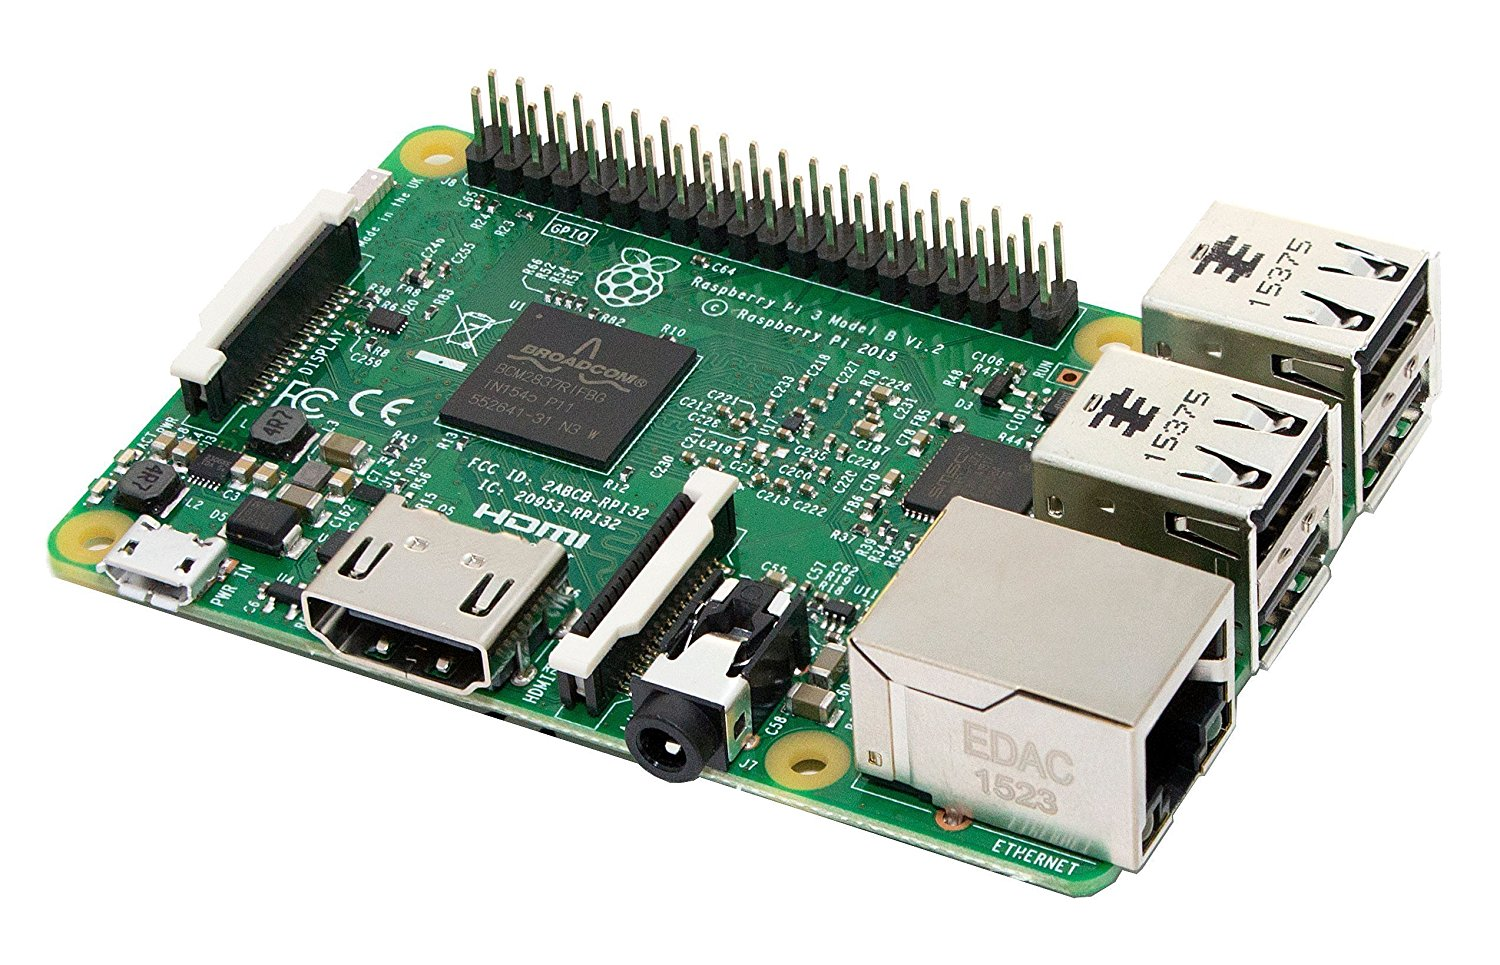
\includegraphics[scale=0.2]{Photos/Raspberry.jpg}
						\caption{Raspberry}
					\end{center}
				\end{figure}
				
		\subsection{Cameras}
			Nous avons 2 caméras qui permettent, l'une la direction (vision frontale) et l'autre la cartographie (vision par dessous). Dans un premier temps, detaillons leur connection entre la Raspberry et le traitement effectué par celle-ci.
			
				\subsubsection{Logitech C170}
					La première est une webcam Logitech C170, que nous avons démonté pour l'assemblage, relié en USB à la Raspberry. 
					\begin{figure}[!h]
					\begin{center}
						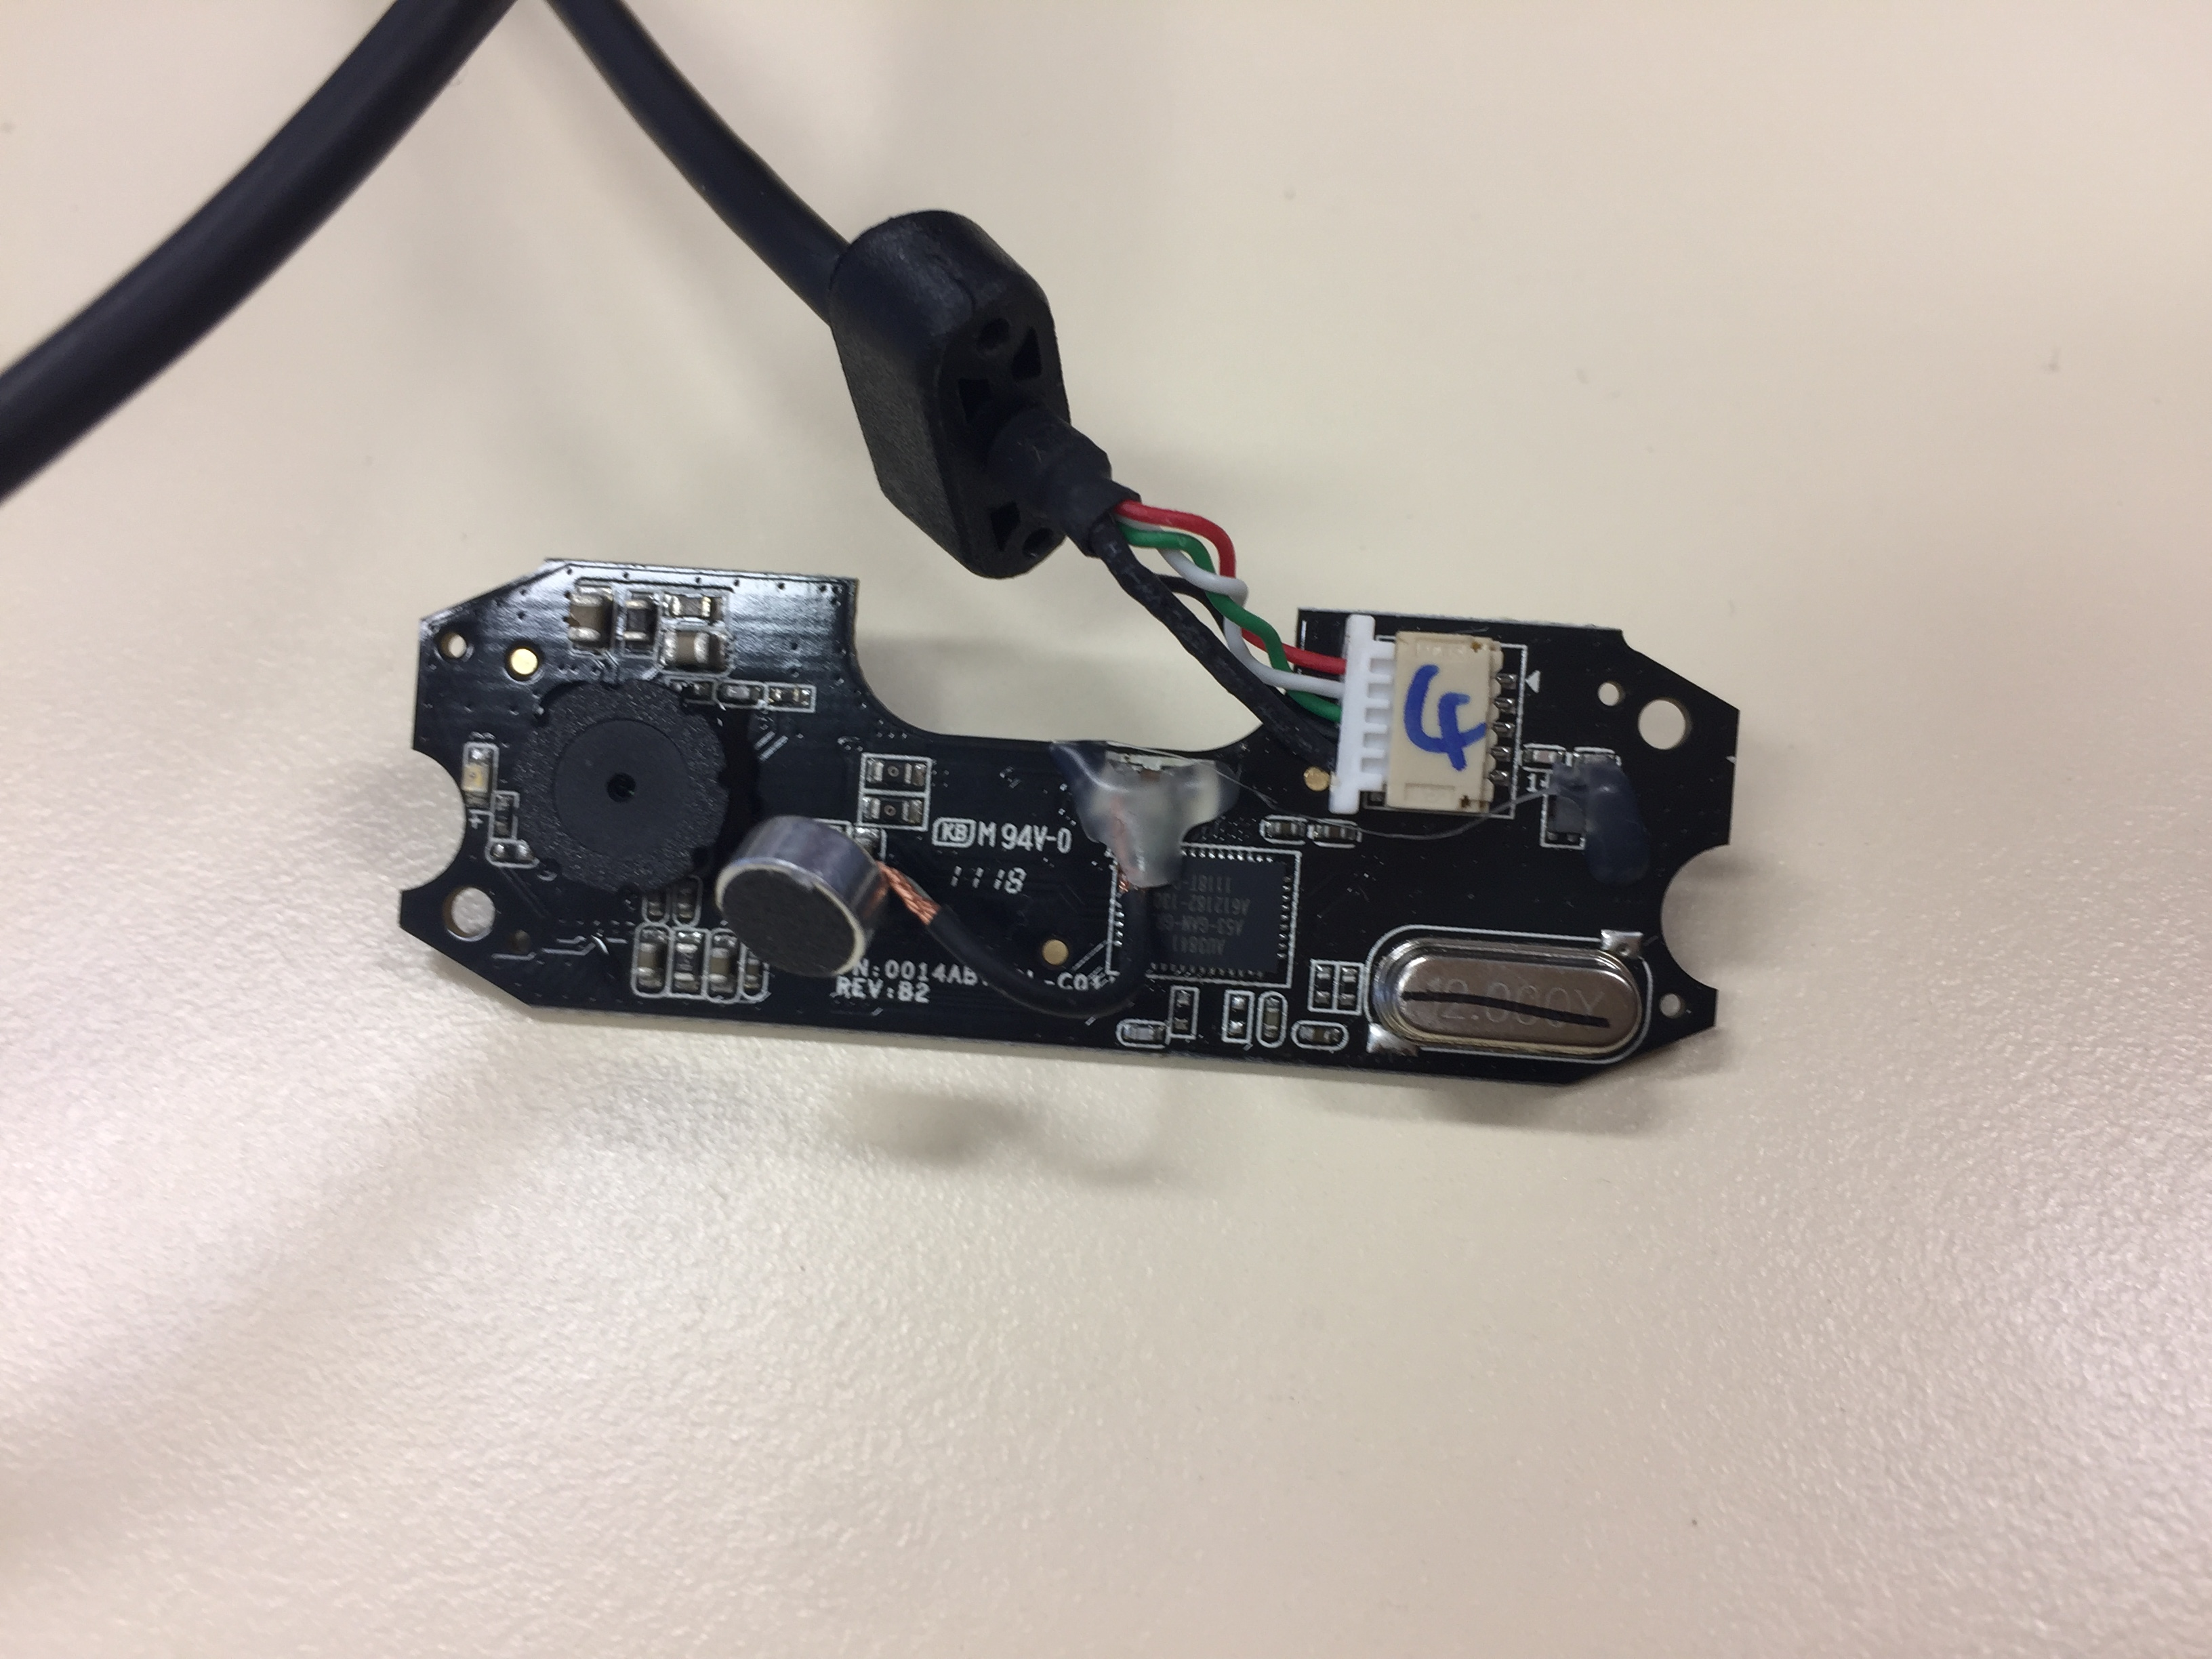
\includegraphics[scale=0.1]{Photos/Camera11.jpg}
						\caption{Logitech C170}
					\end{center}
				\end{figure}
				\newline Nous l'avons choisi car le pilote de celle ci est deja installé nativement sur la Raspberry. Nous utilisons motion qui permet d'envoyer le flux video venant de la camera et de le diffuser en ligne sur notre adresse local \cite{ref1}. En voici le résultat sur un navigateur:
				\begin{figure}[!h]
					\begin{center}
						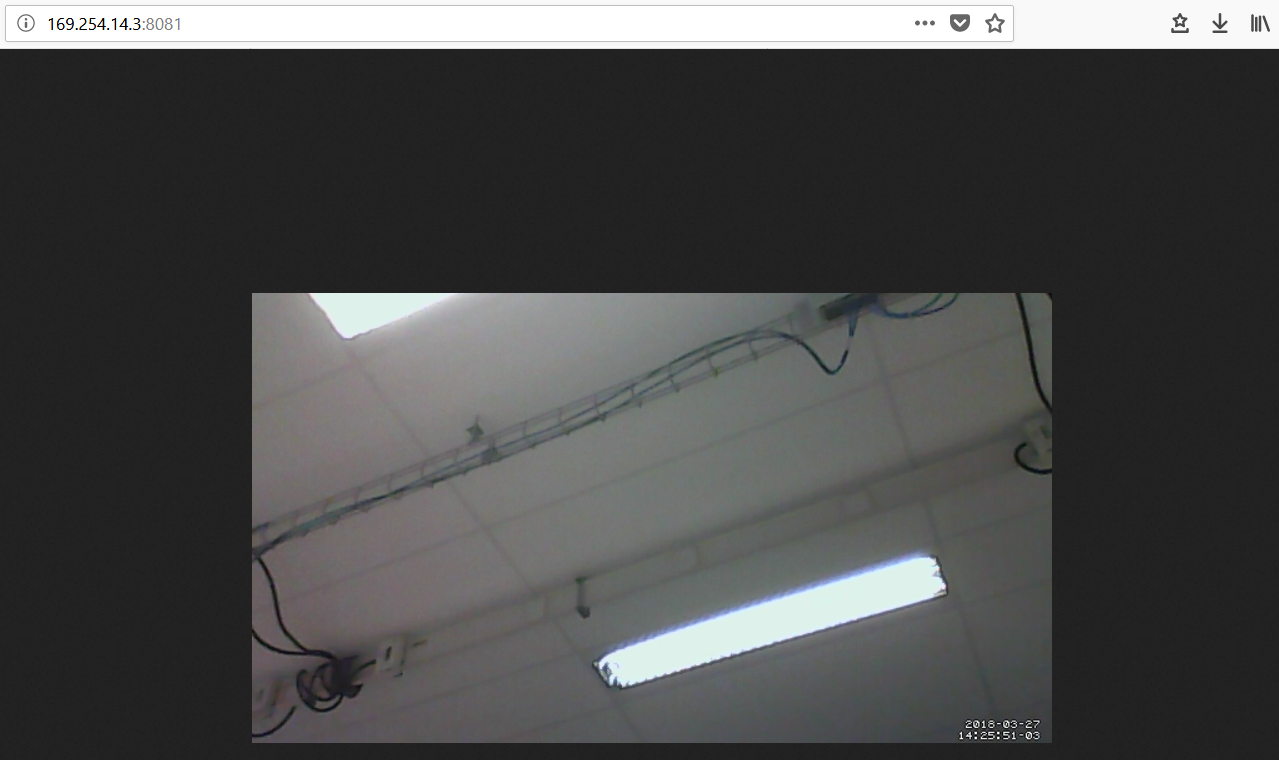
\includegraphics[scale=0.4]{Photos/Camera1.png}
						\caption{Photo Caméra Frontale}
					\end{center}
				\end{figure}
				\newline Cette video sera recuperé par l'interface (expliquer dans le chapitre associé) en 640*360.
				
				\subsubsection{Caméra V2}
					La deuxieme est un module caméra pour raspberry \cite{ref2} qui se raccorde directement par une nappe (un bus de type CSI-2). 
					\begin{figure}[!h]
					\begin{center}
						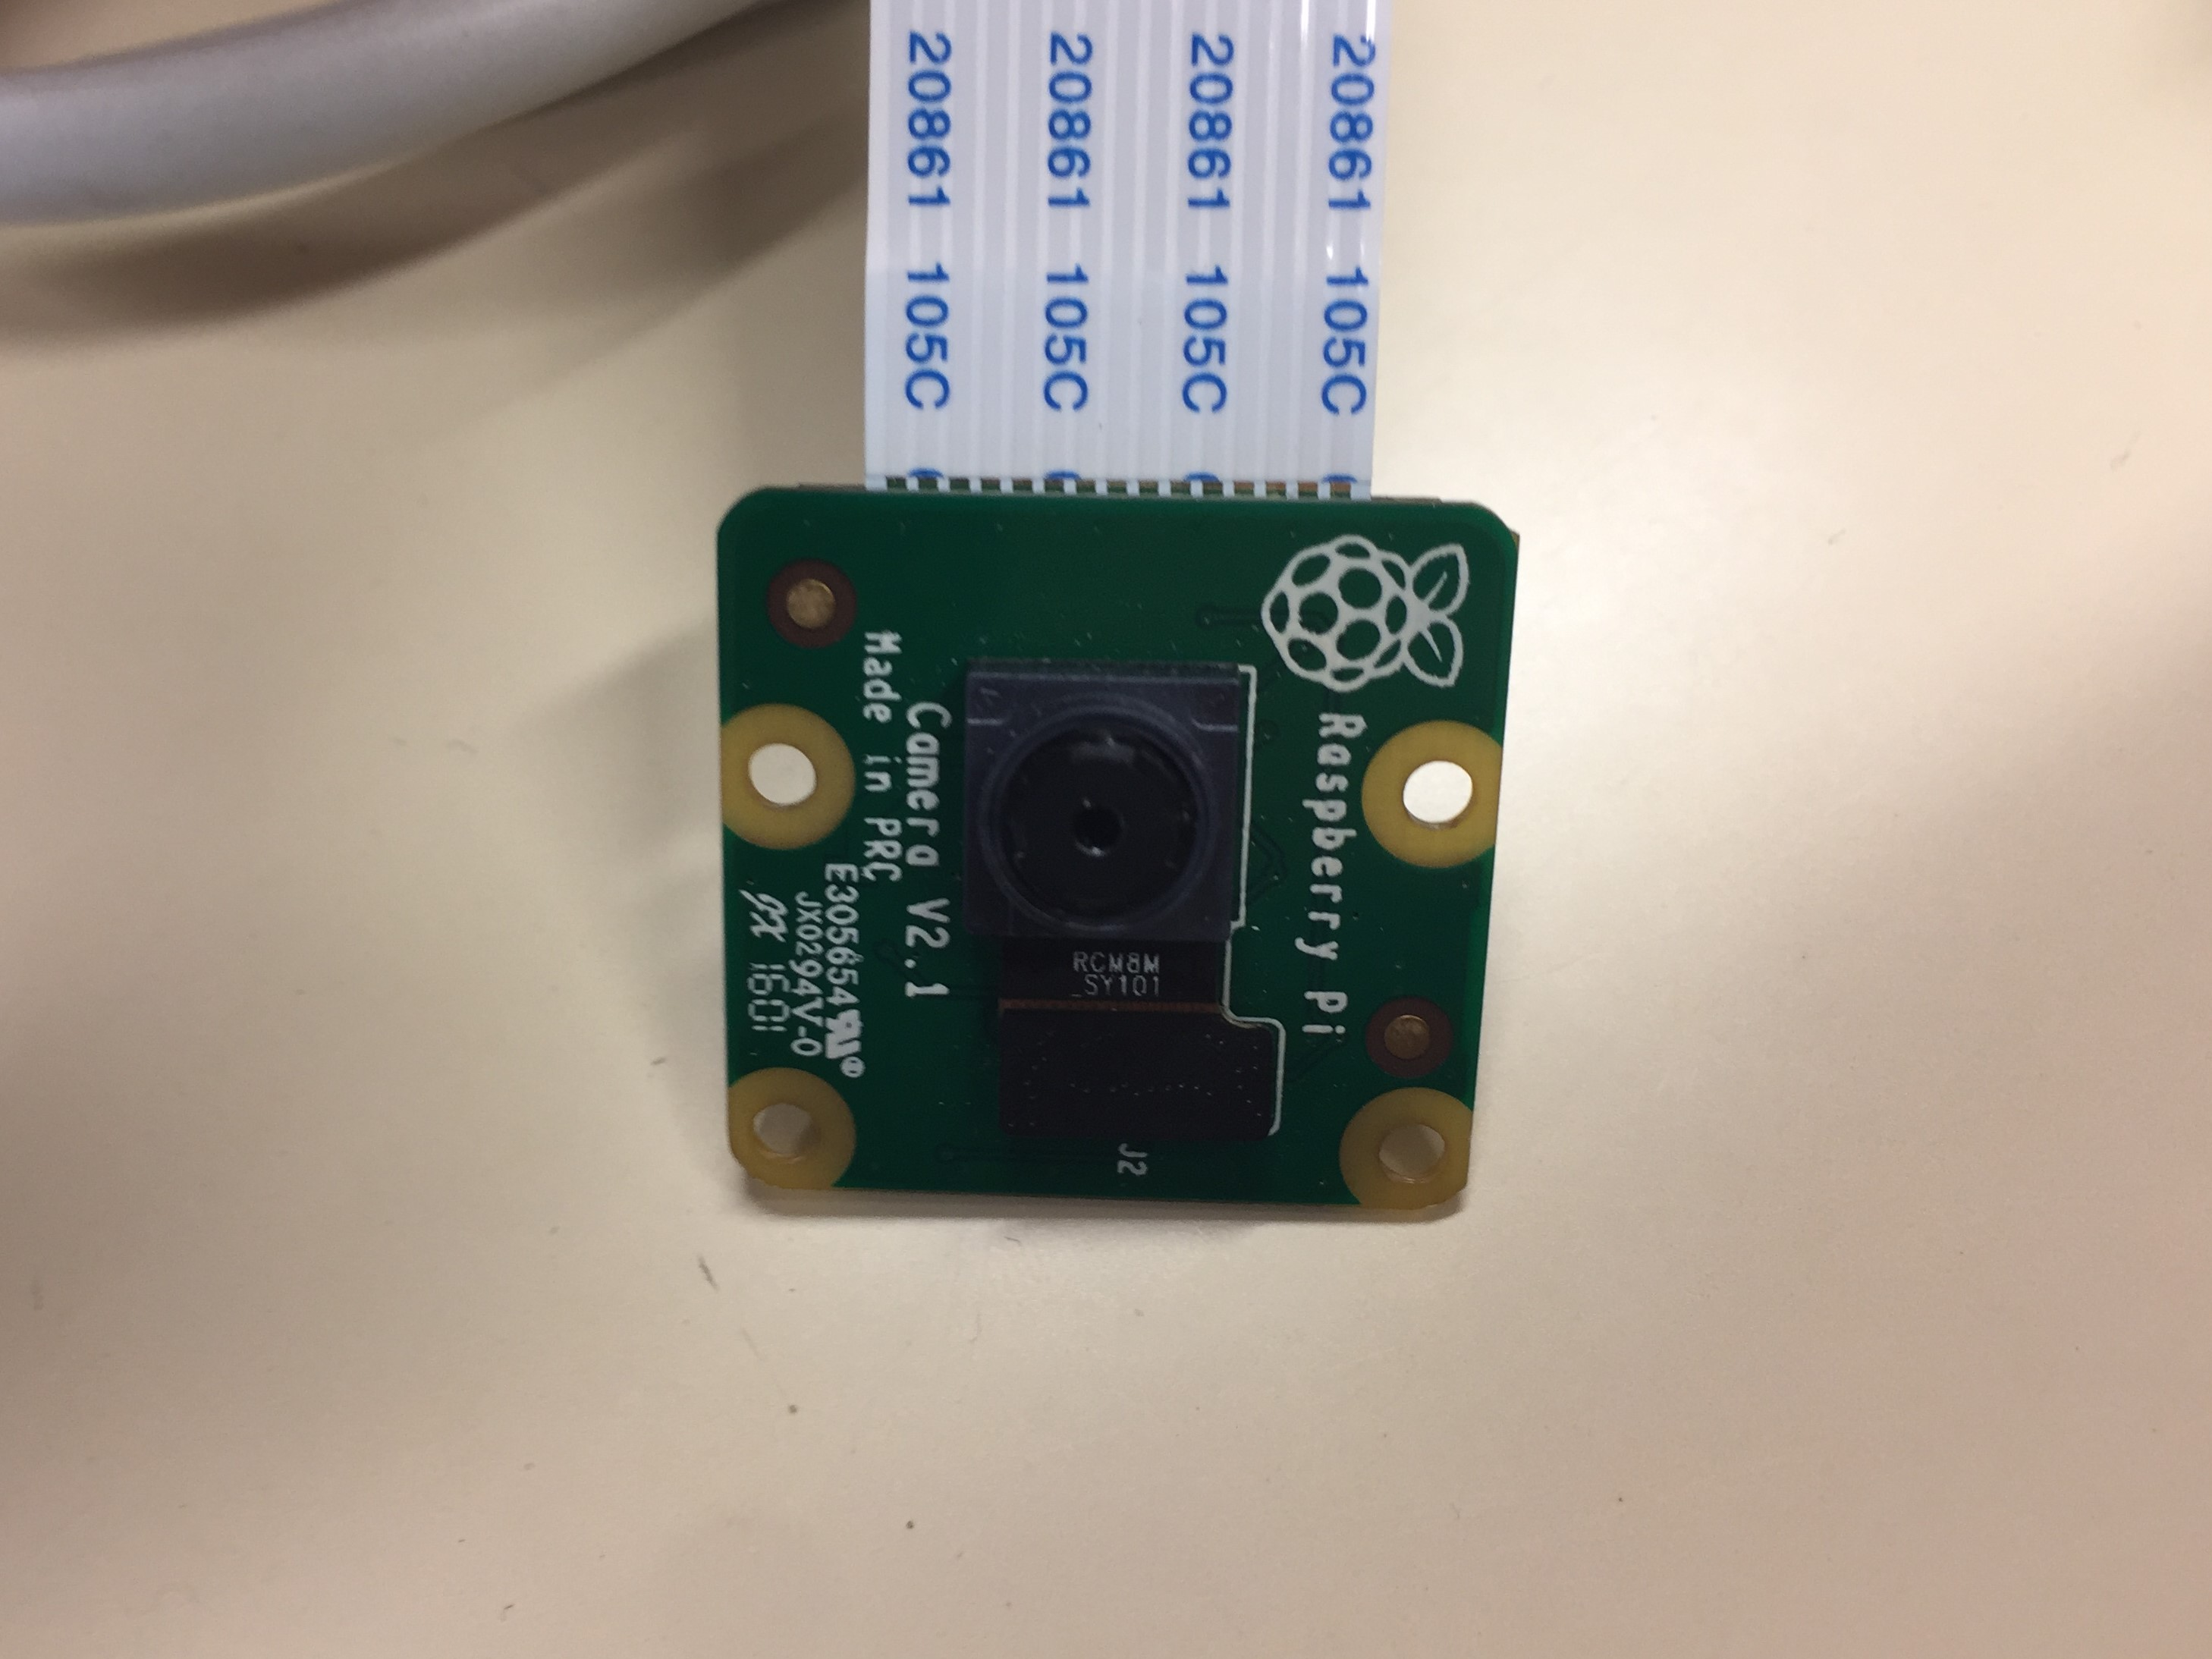
\includegraphics[scale=0.1]{Photos/Camera21.jpg}
						\caption{Module Camera V2 Raspberry}
					\end{center}
				\end{figure}
				\newline Elle se paramètre en python avec les librairies données par le constructeur. De même que l'autre caméra, nous renvoyons un flux video en ligne sur notre adresse local \cite{ref3} mais cette fois-ci sur un autre port.
				\newline
				\newline Le résultat sur un navigateur:
					\begin{figure}[!h]
					\begin{center}
						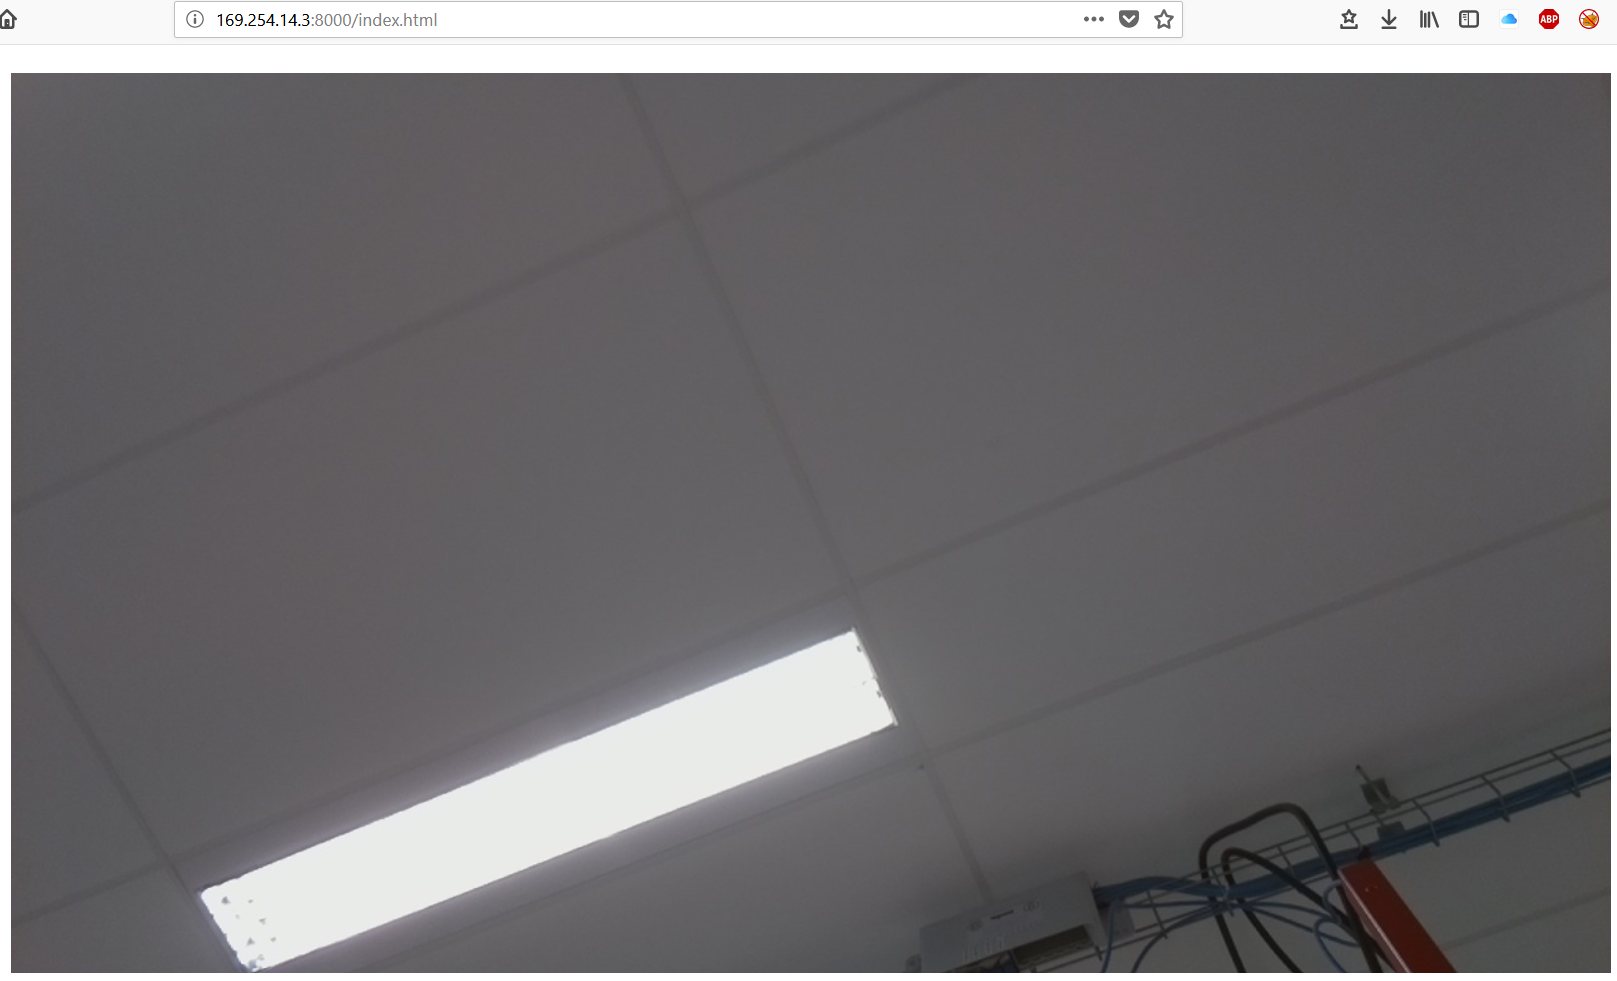
\includegraphics[scale=0.3]{Photos/Camera2.png}
						\caption{Photo Caméra du dessous}
					\end{center}
				\end{figure}
				\newline La video est diffusée en 1920*1080 et affichée par l'interface.
				
		\subsection{Capteur de Pression/Temperature}
		
		\subsection{Central Inertielle}
		Julien
		\newpage
	\section{PC}
		Maintenant que nous avons relié tous nos moteurs, caméras et capteurs à la raspberry ainsi qu'un premier traitement des informations, nous allons voir comment nous traitons cela sur le PC.
		
		\subsection{Interface}
			En premier lieu parlons de l'interface, celle ci à pris differentes formes au cours du temps, ici nous presenterons que la derniere version. Toute la partie PC a été programmé en JAVA \cite{ref4}, l'interface utilise la bibliothèque graphique Swing qui nous permet de gerer l'affichage facilement que ce soit pour la video ou pour les interactions.
			Lorsque l'application est lancé, nous arrivons donc dans un premier menu:
			\begin{figure}[!h]
					\begin{center}
						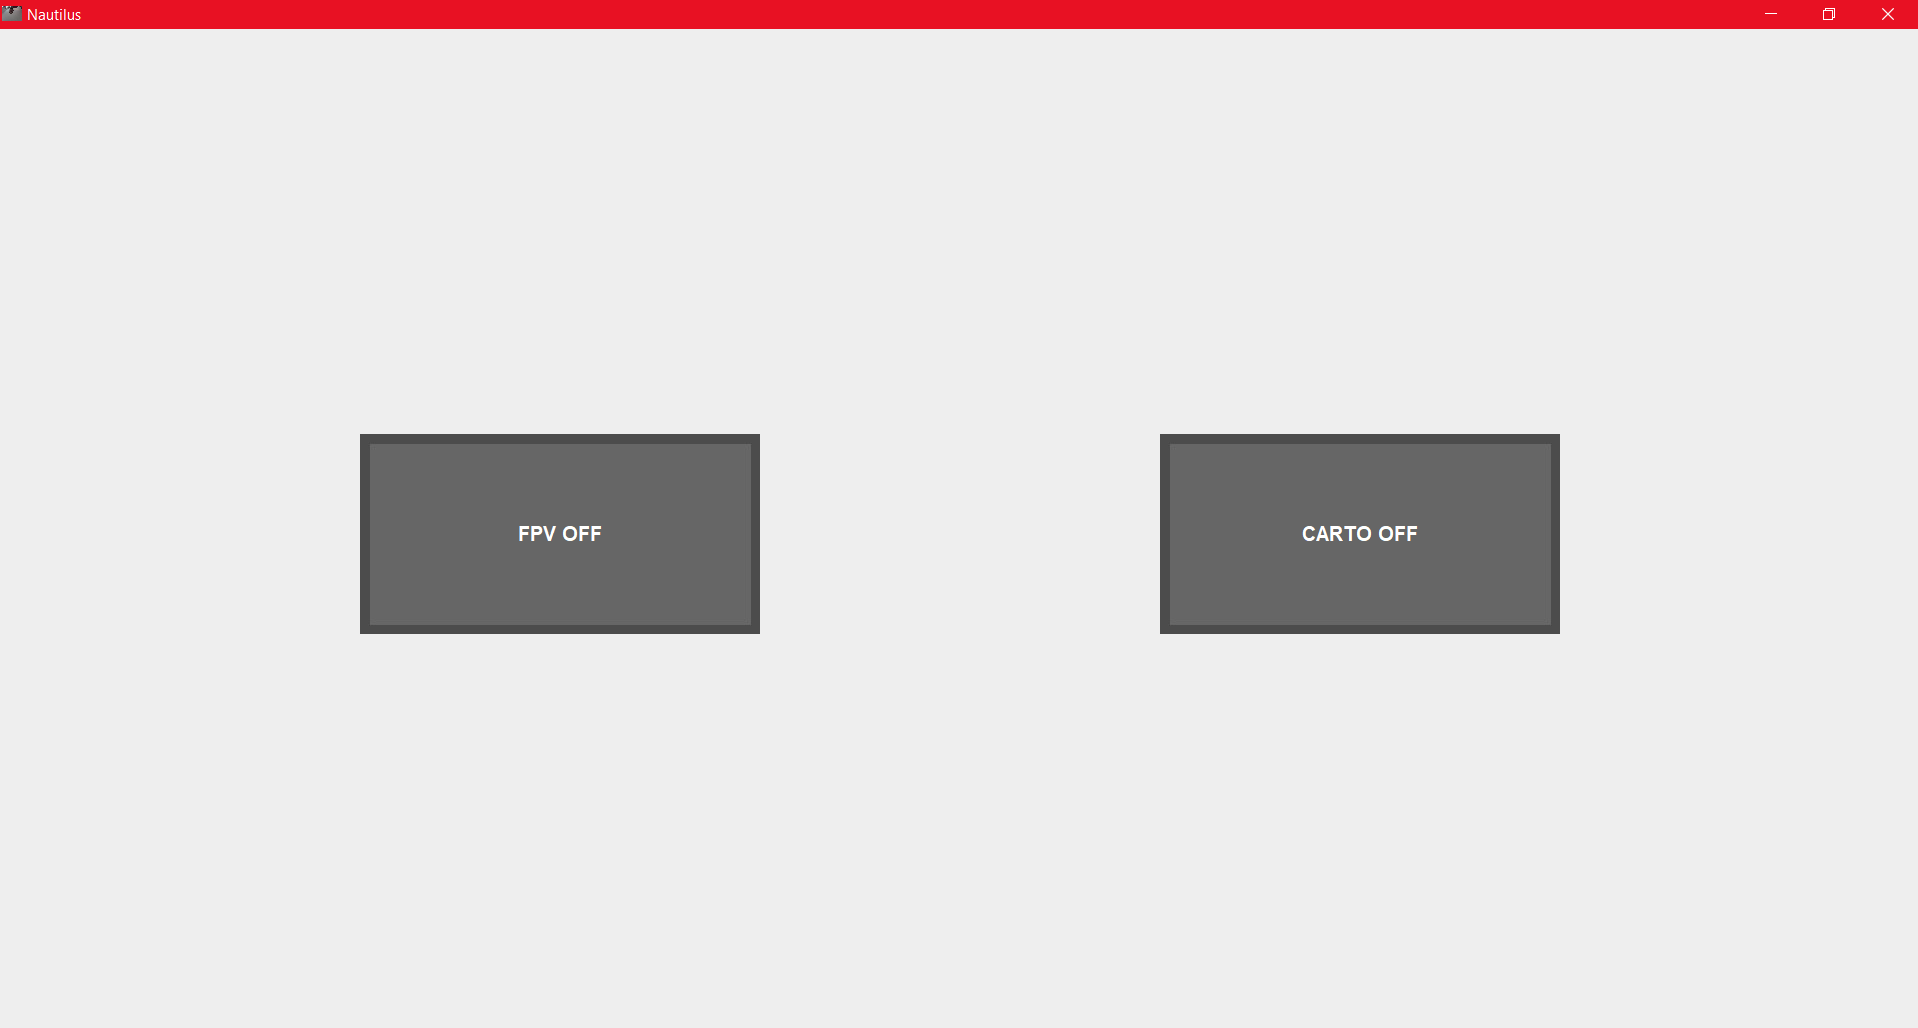
\includegraphics[scale=0.35]{Photos/Interface1.png}
						\caption{Premier Menu Interface}
					\end{center}
				\end{figure}
				\newline Le bouton de Droite mène à une partie que nous developerons dans la partie~\ref{subsec:Cartographie} liée à la Cartographie.
				\newline \newline Nous avons donc crée une fenetre JFrame:
				\begin{lstlisting}[language=java]
Interface inter = new Interface("Nautilus",0,0,1920,1080,true);
				\end{lstlisting}
				Elle est parametrée de façon à prendre tous l'écran, ici 1920*1080, les objets se trouvant dans cette fenetre sont geré pour se placer en fonction de la taille de l'ecran.
				\newline Le manager s'appelle GridBagLayout, il necessite de paramétrer chaque objet.
				Ce manager crée une grille qui se construit en fonction des parametres de chaque objet qu'elle contient.
				\newpage Prenons exemple du premier bouton FPV:
				\begin{lstlisting}[language=java]
axPanel1.setMinimumSize(new Dimension(400,210));
axPanel1.setMaximumSize(new Dimension(400,210));
axPanel1.setPreferredSize(new Dimension(400,210));
c.fill = GridBagConstraints.BOTH;
c.anchor = GridBagConstraints.CENTER;
c.gridx = 0;
c.gridy = 0;
c.weighty = 0.0;
c.weightx = 0.0;
c.gridwidth = 1;
c.gridheight = 1;
c.insets = new Insets(0, 0, 0, 200);
				\end{lstlisting}
				Les 3 premières lignes correspondent à la taille du bouton, que nous avons choisis ici de garder fixe.
				\newline La ligne 4 n'est pas utile dans ce cas mais permet de correctement redimensionner l'objet lorsque la fenetre change de taille.
				\newline La ligne 5 fixe l'objet au centre de la partie qui lui a été alloué.
				\newline La ligne 6 et 7 donne la ligne et la colonne où doit se situé l'objet.
				\newline La ligne 8 et 9 définissent des poids en x et y qui sont utilisé lors d'un redimensionement, cela permet de donner plus de poids à un objet plutot qu'à un autre. Nous ne l'utilisons pas d'où la valeur 0.
				\newline La ligne 10 et 11 permettent de definir combien de ligne et combien de colonne va prendre notre objet.
				\newline La ligne 12 insere une marge dans l'ordre suivant (margeSupérieure, margeGauche, margeInférieur, margeDroite).
				\newline Chaque objet de notre interface est defini de cette façon.
				\newline Ensuite il y a le bouton de Gauche qui lance le systeme complet. Un nouveau menu remplace le précédent:
				\begin{figure}[!h]
					\begin{center}
						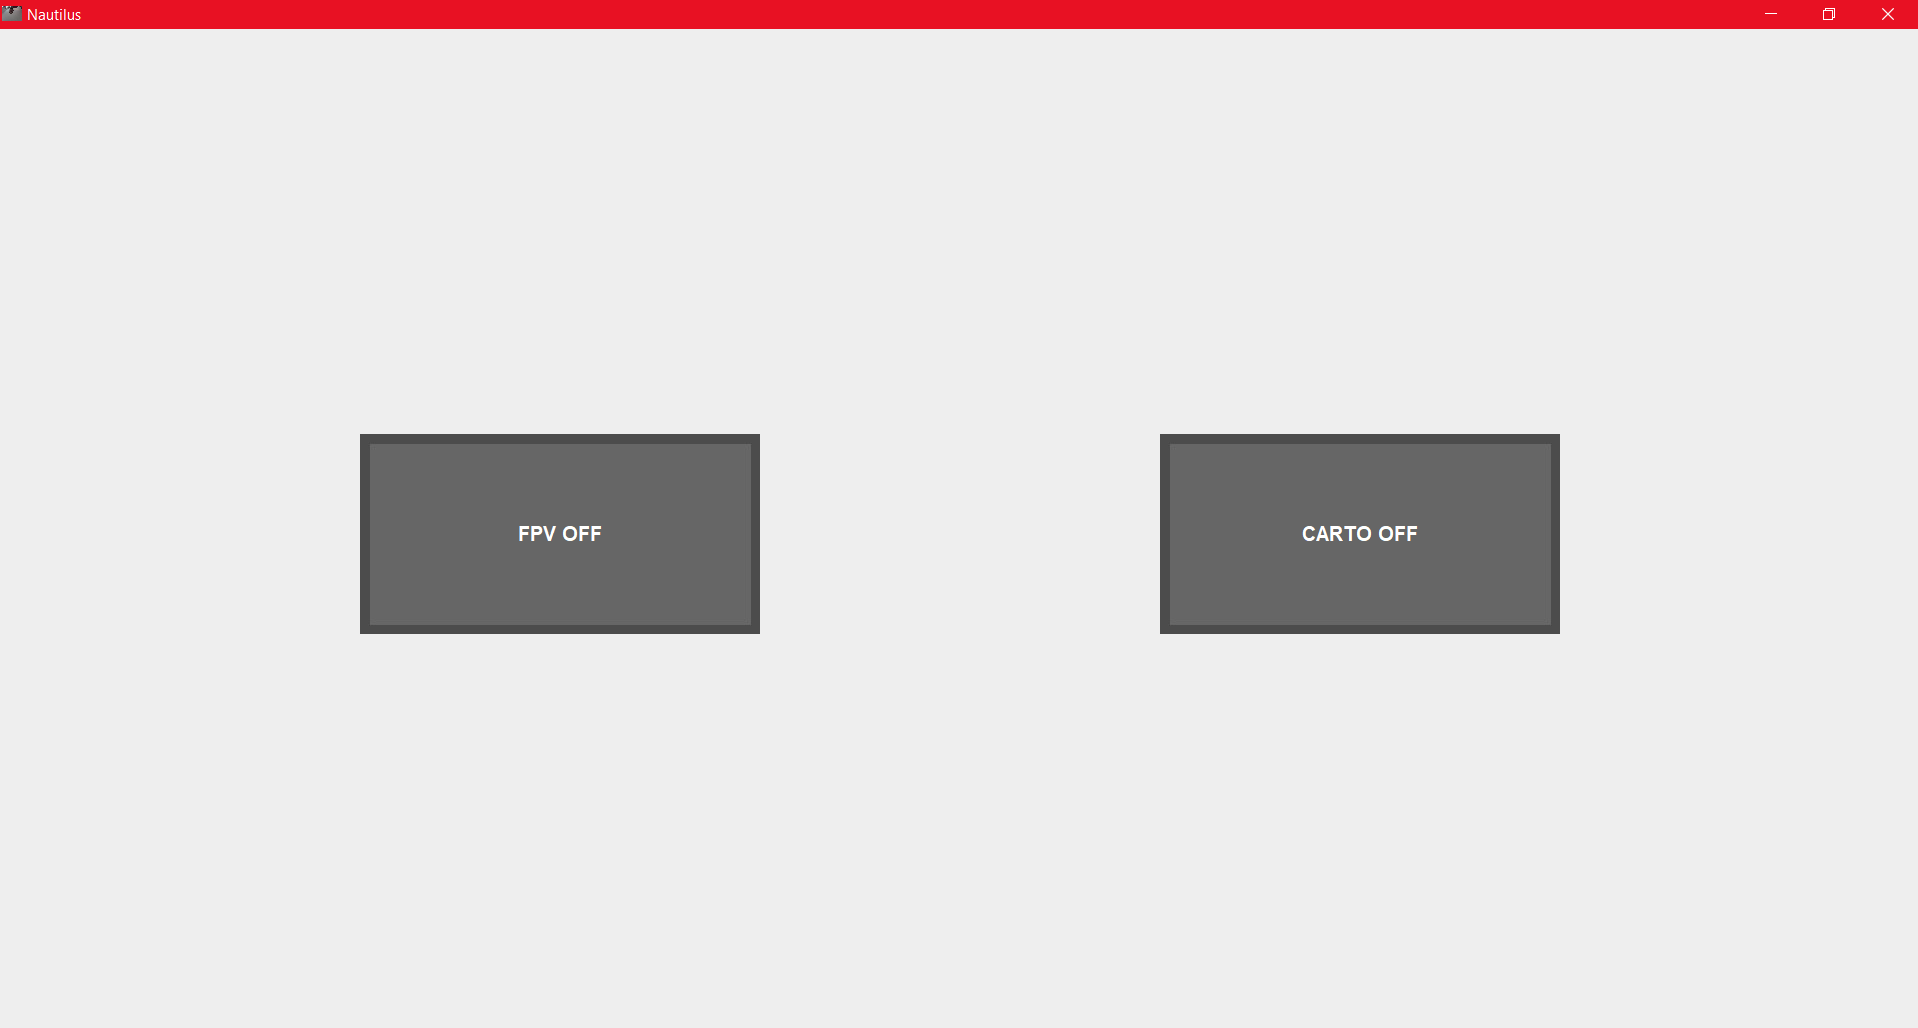
\includegraphics[scale=0.3]{Photos/Interface1.png}
						\caption{Photo Deuxieme menu interface}
					\end{center}
				\end{figure}
				\newline Nous avons maintenant la FPV en haut à gauche, le bouton à droite est le même précédement, les informations des capteurs sont affichées à droite, les commandes envoyées aux moteurs sont en bas et pour finir un affichage 3D (\ref{subsec:Affichage 3D}) avec JAVA3D en bas à droite. Toutes les informations etant actualisées en temps reel avec la Raspberry. Nous allons voir comment.
		\subsection{Tunnel SSH}
			Nous avons choisi d'échanger les données avec la Raspberry par SSH, pour cela on utilise la bibliothèque Jcraft, plus précisement jsch. Au lancement de l'application, il y a 5 tunnels qui se créent (1 pour chaque caméras, 1 pour chaque capteurs et 1 pour les moteurs), ils sont crées au tout debut pour ensuite permettre de transmettre directement les données sans refaire la procédure de connection, le systeme gagne en rapidité. 
			\newline Détaillons maintenant la procédure qui permet de crée ses tunnels. Comme nous sommes en JAVA, une seule classe permet de crée un tunnel et cette classe est ensuite instancié autant de fois que l'on veut.
			\newline Voici le code (Disponible dans /SSH/Exec.java) de création d'un tunnel :
			
			\begin{lstlisting}[language=java]
try{
	JSch jsch=new JSch();
	this.session=jsch.getSession("pi", "169.254.14.03", 22);
	UserInfo ui=new MyUserInfo();
  this.session.setUserInfo(ui);
  this.session.connect();
  this.channel = this.session.openChannel("exec");
  ((ChannelExec)this.channel).setCommand(this.Commande);
  this.channel.setInputStream(null);
  ((ChannelExec)this.channel).setErrStream(System.err);
  this.in=this.channel.getInputStream();
  this.channel.connect();
  byte[] tmp=new byte[1024];
  while(true){
		while(this.in.available()>0){
			int i=this.in.read(tmp, 0, 1024);
      if(i<0)break;
      System.out.print(new String(tmp, 0, i));
      this.retour=new String(tmp, 0, i);
    }
    if(channel.isClosed()){
			if(this.in.available()>0) continue; 
			System.out.println("exit-status: "+channel.getExitStatus());
      break;
     }
   }
}
catch(Exception e){
	System.out.println(e);
}
			\end{lstlisting}
			De la ligne 1 à 5, le tunnel est crée et les informations tel que le nom d'utilisateur, le mot de passe, l'adresse IP et le port sont ajouté aux couches correspondante du tunnel, puis ligne 6 la session est lancé.
		\newline A la ligne 7, nous ouvrons un canal d'execution de commande et ligne 8 nous donnons à ce canal la commande que nous voulons envoyée.
		\newline Les lignes 9,10 et 11 definissent où vont les données entrées, sorties et sorties erreur. Dans notre cas l'entrée ne nous interesse pas car cela passe par une commande, la sortie normal sera stockée et la sortie erreur renvoyé sur l'afficheur d'erreur du systeme (la console). La ligne 12 lance la connection du canal, c'est ici que la commande est envoyée.
		\newline De la ligne 13 à 20 nous permet de récuperer les valeurs retournées par la Raspberry et de les stockées pour ensuite pouvoir les traiter.
		\newline Puis les dernieres lignes, permettent de gerer le cas où le canal est coupé et nous renvoyer d'où vient l'erreur (par exceptions).
		\newline \newline Ces tunnels nous permettent d'envoyer des commandes à la Raspberry et de pouvoir récuperer le retour de cette commande. C'est par ce moyen que nous récuperons presque tous. L'exception étant pour la video IP. Abordons ce sujet.
		\subsection{Videos}
		Nous avons donc 2 flux vidéos à récuperer depuis une adresse IP. Tout d'abord nous devons introduire quelque chse que nous utilisons partout dans notre code: le multi-Thread. Cela permet de lancer plusieurs actions en même temps, c'est ce qu'il se passe avec la récupération des flux videos. Chaque image des flux videos est récuperé puis traité puis affiché en temps reel sans interrompre le reste du programme, tout comme l'envoie de chaque commande.
		\newline Pour les flux videos, c'est une connection http qui est effectué, pour cela la méthode connect est appelée:
		\begin{lstlisting}[language=java]
public void connect()
	{
		try
		{
			URL u = new URL(useMJPGStream?mjpgURL:jpgURL);
			huc = (HttpURLConnection) u.openConnection();
			InputStream is = huc.getInputStream();
			connected = true;
			BufferedInputStream bis = new BufferedInputStream(is);
			dis= new DataInputStream(bis);
			if (!initCompleted) initDisplay();
		}
		catch(IOException e)
		{ //Relance la connection si pas de connection en attendant 60 sec
			try
			{
				huc.disconnect();
				Thread.sleep(60);
			}
			catch(InterruptedException ie)
			{
				System.out.println(ie);
			}
		}
		catch(Exception e){;}
	}
			\end{lstlisting}
			De la ligne 5 à 10, la procédure de connection http est effectué.
			\newline Après la ligne 12, on gère les execeptions liées à la connection.
			\newline A la ligne 10, les données récuperées sont stockées dans une variable globale à Caméra.
			\newline Les informations vont être ensuite traité par initDisplay qui est appelé en ligne 11.
			\newline Observons cette méthode :
		\begin{lstlisting}[language=java]
public void initDisplay()
	{ 
		if (useMJPGStream)readMJPGStream();
		else
		{
			readJPG();
			disconnect();
		}
		imageSize = new Dimension((image.getWidth(this)*2), image.getHeight(this)*2);
		setPreferredSize(imageSize);
		parent.validate();
		initCompleted = true;
	}
		\end{lstlisting}
		Le premier If/Else permet de distinguer le cas où le flux serait videos ou juste photo. Dans notre cas c'est un flux videos composé d'image JPG.
		\newline Le reste de la méthode permet de preparé l'affichage des images.
		\newline Nous somme toujours dans la procedure de connection, la lecture de la premiere image récuperé est fait. Pour cela la méthode readMJPGStream qui appel readJPG permet de décoder l'image et de la stocké dans la variable image. Voici les 2 méthodes :
		\begin{lstlisting}[language=java]
public void readMJPGStream()
	{
		readLine(4,dis); //enleve les 3 premieres lignes
		readJPG();
		readLine(1,dis); //enleve les 2 dernieres lignes
	}
	
public void readJPG()
	{
		try{
			JPEGImageDecoder decoder = JPEGCodec.createJPEGDecoder(dis);
			image = decoder.decodeAsBufferedImage();
		}catch(Exception e){
			disconnect();
		}
	}
		\end{lstlisting}
		La procédure de decodage d'une image JPEG est faite par une bibliothèque externe.
		\newpage Après cette procédure de connection, les 2 méthodes ci dessus sont appelé en boucle et l'affichage mis à jour:
		\begin{lstlisting}[language=java]
public void readStream()
	{
		try{
			if (useMJPGStream){
				while(true){
					readMJPGStream();
					parent.repaint();
				}
			}
    	}catch(Exception e){;}
    }
		\end{lstlisting}
		L'affichage étant geré par la bibliothèque Swing, c'est la méthode paint() qui affiche l'image et de plus trace une ligne qui en fonction des angles d'euler renvoyé par la centrale intertiel :
		\begin{lstlisting}[language=java]
public void paint(Graphics g)
	{
		if (image != null)
			image=scale(image, 2);
			g.drawImage(image, 0, 0, this);
			Graphics2D g2 = (Graphics2D) g;
			double alpha = Interface.rotZ* Math.PI/180f;
    	int a = image.getHeight();
    	int b = image.getWidth();
    	double S =(b/2)*(Math.sin(alpha))*(Math.cos((Math.PI/2)-alpha));
    	double T =(b/2)*(Math.sin(alpha))*(Math.sin((Math.PI/2)-alpha));
    	g2.draw(new Line2D.Double(S,(a/2)-T,b-S,(a/2)+T));
	}
		\end{lstlisting}
	L'image est redimensionnée pour le bien de l'affichage et la ligne est tracé avec 2 points calculé par rapport à une rotation avec une origine au centre de l'image.
	\newline \newline Nos 2 flux videos sont donc récuperés et peuvent donc être appelés par un JPanel n'importe où.
\newpage
		\subsection{Capteurs et Moteurs}
		\subsubsection{Capteurs}
		Nous avons deja precedement préparé la raspberry pour qu'elle renvoit les informations que l'on veut en fonction d'une commande. Il nous suffit maintenant d'envoyer en temps reel et en boucle infini les commandes (capteur de pression et centrale inertielle) grâce au systeme de multi-thread.
		\newline Expliquons la méthode pour le capteur de pression. Tout d'abord il faut crée le thread lié à la classe qui sera executer en boucle, puis on lance le thread avec la méthode, ce qui donne :
		\begin{lstlisting}[language=java]
Pression ex4 = new Pression();
Thread a4 = new Thread(ex4);
a4.start();
		\end{lstlisting}
		La classe Pression doit être héritière de Runnable pour permettre le lancement en thread.
		\newline Observons dans la classe Pression, la méthode start:
		\begin{lstlisting}[language=java]
Interface.exPression.Commander("python MS5803_14BA.py");
String[] a = Interface.exPression.retour.split("/");
this.Pression=a[0];
this.TemperatureC=a[1];
this.TemperatureF=a[2];
Interface.pre=Pression;
Interface.tempC=TemperatureC;
Interface.tempF=TemperatureF;
Interface.pression.setText(" Pression = "+Interface.pre);
Interface.pression.repaint();
Interface.temperatureC.setText(" TemperatureC = "+Interface.tempC);
Interface.temperatureC.repaint();
Interface.temperatureF.setText(" TemperatureF = "+Interface.tempF);
Interface.temperatureF.repaint();
		\end{lstlisting}
		Nous commençons en ligne 1 par envoyer la commande grâce au tunnel précédement crée pour le capteur de Pression puis nous récuperons les valeurs sous forme de chaînes de caracteres.
		\newline Enfin nous mettons à jour les valeurs globales et l'affichages.
		
		\subsubsection{Moteurs}
		Pour les moteurs, on envoi juste une commande à la Raspberry :
		\begin{lstlisting}[language=java]
Interface.exMoteur.setCommande("echo 0="+m1+" > /dev/servoblaster & echo 1="+m2+" > /dev/servoblaster & echo 2="+m3+" > /dev/servoblaster");
Thread a1 = new Thread(Interface.exMoteur);
a1.start();
while( a1.isAlive()) {}
Interface.m1=this.m1;
Interface.m2=this.m2;
Interface.m3=this.m3;
Interface.moteur1.setText(""+Interface.m1+"    ");
Interface.moteur1.repaint();
Interface.moteur2.setText(""+Interface.m2+"    ");
Interface.moteur2.repaint();
Interface.moteur3.setText(""+Interface.m3+"    ");
Interface.moteur3.repaint();
		\end{lstlisting}
		On oublie pas de mettre à jour au passage l'affichage.
		\newline Ce code est donc execter à chaque fois que l'on appuie sur une des touches de directions.
		\newline Nous avons défini les touches suivantes:
		\newline Monter/Descente : Z/S
		\newline Gauche/Droite : Flêche Gauche/Droite
		\newline Monter/Descente : Z/S
		\newline Arrete d'urgence : Barre Espace
		
		\subsection{Affichage 3D}
			\label{subsec:Affichage 3D}
			Nous utilisons JAVA3D pour afficher le modele qui est extrait de Solidworks.
			\newline Tout d'abord nous devons crée un canvas 3D qui contiendra notre objet 3D et nous l'inserons au mileux d'un JPanel :
		\begin{lstlisting}[language=java]
Canvas3D canvas3D = new Canvas3D(SimpleUniverse.getPreferredConfiguration());
this.add(canvas3D, BorderLayout.CENTER);
		\end{lstlisting}
		Puis nous créons un simple univers qui contient notre canvas3D.
		\newline Nous devons maintenant positionner notre point d'observation pour avoir une vu correcte:
		\begin{lstlisting}[language=java]
OrbitBehavior orbit = new OrbitBehavior(canvas3D, OrbitBehavior.REVERSE_ROTATE);
orbit.setRotXFactor(0);//or any other value
orbit.setRotYFactor(0);
orbit.setTransXFactor(0);
orbit.setTransYFactor(0);
orbit.setSchedulingBounds(new BoundingSphere());
simpleU.getViewingPlatform().setViewPlatformBehavior(orbit);
ViewingPlatform vp = simpleU.getViewingPlatform();
TransformGroup steerTG = vp.getViewPlatformTransform();
Transform3D t3d = new Transform3D();
steerTG.getTransform(t3d);
t3d.lookAt(new Point3d(-1.2,1.2,1.2), new Point3d(0,0,0), new Vector3d(0,1,0));
t3d.invert();
steerTG.setTransform(t3d);
		\end{lstlisting}
		De la ligne 1 à 6, nous definissions un mouvement orbital de la caméra puis pour le moment nous fixons les rotations et les translations (on pourra les debloquer si on le veut)
		\newline Les lignes 9 à 14 permettent de definir la position initiale de notre point d'observation.
		\newline Nous devons ensuite crée ce qu'on appele une scene, c'est dans cette scene que tous nos objets 3d se trouveront:
		\begin{lstlisting}[language=java]
BranchGroup scene = createSceneGraph(simpleU);
scene.compile();
simpleU.addBranchGraph(scene);
		\end{lstlisting}
		Les 2 ligns suivant compile la scene et rattache notre scene à l'univers.
		\newline \newline Maintenant nous devons crée cette scene 3d qui contiendra notre objet mais aussi la lumière, notre eau fictive et les mouvements possible.
		\newline Tous ce passe dans la méthode createSceneGraph.
		\begin{lstlisting}[language=java]
public BranchGroup createSceneGraph(SimpleUniverse simpleU) 
	{
    BranchGroup parent = new BranchGroup();
    BoundingSphere bounds = new BoundingSphere(new Point3d(), 100);
    Light ambientLight = new AmbientLight(new Color3f(Color.white));
    ambientLight.setInfluencingBounds(bounds);
    parent.addChild(ambientLight);
		
    Light directionalLight = new DirectionalLight(
      new Color3f(Color.white),
      new Vector3f(1, -1, -1));
    directionalLight.setInfluencingBounds(bounds);
    parent.addChild(directionalLight);
		\end{lstlisting}
		La ligne 3 crée un objet parent qui contiendra tous nos objets.
		\newline De la ligne à 4 à 7, on crée une lumiere ambiante de couleur blanche
		\newline Puis de la ligne 9 à la ligne 13, une lumiere directionnel pour augmenter la luminosité dans la même direction que notre point d'observation.
		\newline Nous ne detaillerons pas ici le code de la création de l'eau, le principe étant qu'on a crée 4 plans positionnés correctement autour du ROV et on lui applique une textures bleu (que l'on peut changer facilement). Et on oublie pas de l'ajouter à l'objet parent.
		\newline Maintenant autorisons les mouvements de la souris pour notre objet :
		\begin{lstlisting}[language=java]
TransformGroup mouseTransform = new TransformGroup();
mouseTransform.setCapability(TransformGroup.ALLOW_TRANSFORM_READ);
mouseTransform.setCapability(TransformGroup.ALLOW_TRANSFORM_WRITE);
mouseTransform.addChild(loadWavefrontObject());
		\end{lstlisting}
		Et en ligne 4 nous ajoutons notre ROV. La méthode loadWavefrontObject() permet de recuperer un objet 3D à partir d'un fichier .obj.
		\newline Pour la fin de cette méthode, les commentaires decrivent les opérations effectués
		\begin{lstlisting}[language=java]
// Creation de l'homethetie (homothetie)
Transform3D homothetie = new Transform3D();
homothetie.setScale(Interface.scale); 
    
// Creation de la transformation (translation)
 Transform3D translation = new Transform3D();
translation.setTranslation(new Vector3f(0f, 0f, 0f));
translation.mul(homothetie);
    
// Creation de la rotation X(rotation)
Transform3D rotationX = new Transform3D();
rotationX.rotX( Interface.rotX * Math.PI/180f);
rotationX.mul(translation);
    
// Creation de la rotation Y(rotation)
Transform3D rotationY = new Transform3D();
rotationY.rotY( Interface.rotY * Math.PI/180f);
rotationY.mul(rotationX);
    
// Creation de la rotation Z(rotation)
Transform3D rotationZ = new Transform3D();
rotationZ.rotZ( Interface.rotZ * Math.PI/180f);
rotationZ.mul(rotationY);
    
this.rotationGroup = new TransformGroup(rotationZ);

//Autorisation de modifier les transformations
rotationGroup.setCapability(TransformGroup.ALLOW_TRANSFORM_READ);
rotationGroup.setCapability(TransformGroup.ALLOW_TRANSFORM_WRITE);
    
// Ajout au graphe de la scene
rotationGroup.addChild(mouseTransform);
parent.addChild(rotationGroup);

return parent;
		\end{lstlisting}
		Notre scene renvoie donc tous les objets qu'on a crée précédement.
		\newline \newline Maintenant nous voulons que notre ROV 3D soit capable de se mouvoir en fonction des angles d'euler renvoyer et stocker dans notre interface.
		\newline Pour cela on a crée une méthode mouvement:
		\begin{lstlisting}[language=java]
public void mouvement(double rotX, double rotY, double rotZ, Vector3d trans, double scale)
		\end{lstlisting}
		Elle prend donc en argument, les 3 rotations, un vecteur des translations (sur tous les axes) et un paramêtre multiplicateur d'echelle.
		\newline Cette méthode modifie la matrice 4*4 contenant la matrice de rotation, translation et de mise à l'echelle.
		\newline Puis effectue les transformations de cette matrice.
		
		\subsection{Cartographie}
			\label{subsec:Cartographie}
			Cette partie n'a pas été beaucoup developpé mais un premier systeme a été crée mais pas intégré dans la dernière version de l'interface.
			\newline Grâce à l'appuie sur une touche, une photo de la camera du dessous est enregistrer dans un dossier. Voici le code qui permet d'enregistrer notre photo en jpg :
			\begin{lstlisting}[language=java]
BufferedImage img = new BufferedImage(axPanel.getWidth(), axPanel.getHeight(), BufferedImage.TYPE_INT_RGB);
axPanel.print(img.getGraphics());
try {
	ImageIO.write(img, "jpg", new File(nomPhoto+".jpg"));
}
catch (IOException e5) {
	e5.printStackTrace();
}
		\end{lstlisting}
			Le systeme n'est pas fini mais dans l'absolu chaque photo serai enregistrer avec un nom different avec les données de localisation dans les meta-données de la photo.
			\newline Ensuite il y a un autre bouton (non affiché sur la derniere interface) qui ouvre une autre fenetre avec toute nos photos positionnées, en fonction des coordonnées GPS, sur une carte.
			\newline On peut cliquer sur chaque photo pour les agrandir dans une nouvelle fenetre.
			\newline Tous les codes se trouvent dans le sous-dossier /Carto.
			
\chapter{Conclusion}
			
\chapter{Références}

				\textbf{Motorisation et énergie :}
				\begin{itemize}
							\item \textbf{\href{http://www.conrad.fr/ce/fr/product/231891/Moteur-davion-lectrique-brushless-ROXXY-315079?ref=searchDetail}{Référence 1}} : Moteur d'avion électrique brushless ROXXY 315079 chez Conrad (x3)
							\item \textbf{\href{https://www.robotshop.com/eu/fr/esc-multirotor-20a-m20a.html}{Référence 2}} : ESC Suppo Multirotor 20A M20A chez RobotShop (x3)
							\item \textbf{\href{https://hobbyking.com/fr_fr/hobbykingr-tm-brushless-car-esc-30a-w-reverse.html}{Référence 3}} : ESC HobbyKing 30A avec Reverse (x1)
							\item \textbf{\href{https://www.topmodel.fr/product-detail-18656-graupner-mx-20-hott-12160?lang=fr}{Référence 4}} : Radiocommande Graupner MX-20 (disponible à l'ENSEA)
							\item \textbf{\href{http://www.conrad.fr/ce/fr/product/206028/Batterie-daccumulateurs-NiMh-72-V-3000-mAh-Conrad-energy-206028-stick-fiche-Tamiya-mle?ref=searchDetail}{Référence 5}} : Batterie d'accumulateurs (NiMh) 7.2 V 3000 mAh Conrad (x1)
				\end{itemize}

\bibliographystyle{unsrt} % Le style est mis entre accolades.

\bibliography{bibliographie} % mon fichier de base de données s'appelle bibli.bib

\listoffigures

\end{document}
